\section{Leis de Kirchhoff}

A \textbf{primeira lei de Kirchhoff} fala sobre as correntes em um nó, por isso é comum ser chamada de \textbf{lei dos nós}, enquanto que a \textbf{segunda lei de Kirchhoff} fala sobre as tensões em uma malha, sendo assim a \textbf{lei das malhas}.


\subsection{1ª Lei de Kirchhoff}

\textbf{A soma das correntes em um nó é igual a zero.}

\begin{figure}[!h]
	\centering
	\caption{Circuito em paralelo}
	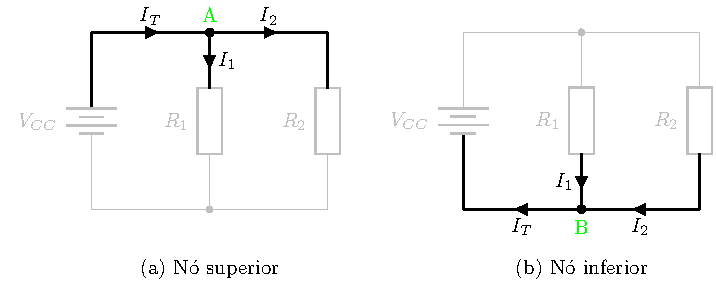
\includegraphics[scale=1.0]{fig-noSupInf}
	\label{fig:nosAeB}
\end{figure}


A Figura \ref{fig:nosAeB} mostra o sentido convencional da corrente nos dois nós do circuito.

Tendo um nó como referência, adota-se uma convenção para o sentido da corrente. Assim, a corrente que chega ao nó é anotada como positiva e a corrente que sai é negativa. O oposto também pode ser adotado.

Escrevendo, pela definição, a equação para o nó $A$ temos:

\begin{eqnarray}
\label{eq:1kirchhoff}
(+I_T) + (-I_1) + (-I_2) & = & 0\\
I_T - I_1 - I_2 & = & 0 \nonumber\\
I_T - I_1 - I_2 \color{blue}{+ I_1 + I_2}& = & 0 \color{blue}{+I_1 + I_2} \nonumber\\
I_T \cancel{-I_1} \cancel{- I_2} \color{blue}{\cancel{+ I_1} \cancel{+ I_2}}& = & \color{blue}{+I_1 + I_2} \nonumber\\
I_T = I_1 + I_2
\end{eqnarray}

Da mesma forma para o nó $B$:
\begin{eqnarray}
(-I_T) + (+I_1) + (+I_2) & = & 0 \nonumber\\
-I_T + I_1 + I_2 \color{blue}{+I_T}& = & 0\color{blue}{+I_T} \nonumber\\
\cancel{-I_T} + I_1 + I_2 \color{blue}{\cancel{+I_T}}& = & 0\color{blue}{+I_T} \nonumber\\
I_1 + I_2 & = & I_T \nonumber
\end{eqnarray}










\subsection{A divisão da corrente no nó}

A intensidade da corrente que circula em um ramo, depende da tensão aplicada aos seus nós e da resistência total do ramo. Assim, para o circuito da Figura \ref{fig:paralelo} (a) a corrente total depende apenas do valor de $V_{CC}$ e $R_1$.

Não havendo mudanças em $V_{CC}$ ou $R_1$, não haverá mudança no valor da intensidade de corrente, denotada $I_T$. A intensidade da corrente que flui da fonte é a mesma que atravessa a carga, com uma certa resistência e condutância.

Ao inserir outro ramo ao circuito, como mostrado na Figura \ref{fig:paralelo}(b), a intensidade da corrente no ramo de $R_1$ não é alterado, pois a tensão entre os pontos $A$ e $B$ não muda, bem como seu valor ôhmico, porém, a intensidade total da corrente muda, pois há agora um novo caminho, um novo ramo para circulação da corrente.

\begin{figure}[!h]
	\centering
	\caption{Circuito em paralelo}
	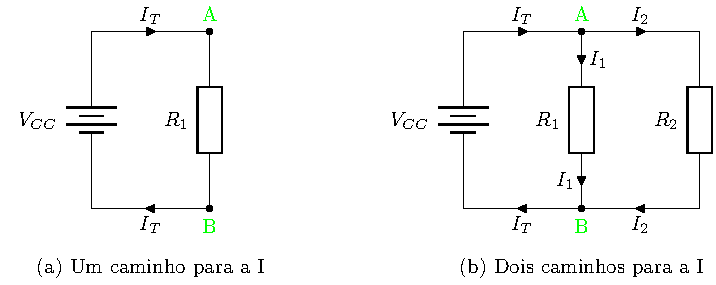
\includegraphics[scale=1.0]{fig-paralelo}
	\label{fig:paralelo}
\end{figure}

A mudança do circuito (a) para o (b), do ponto de vista da corrente, produz um novo caminho para a circulação da corrente. Pode-se dizer então que com a inclusão do novo ramo, conectado aos mesmos pontos do ramo já existente, há agora uma maior facilidade para a corrente fluir, pois agora são dois caminhos.

Podemos obter a condutância total do circuito paralelo somando as condutâncias dos ramos, da seguinte forma:

\begin{eqnarray}
  G_T & = & G_{R_1} + G_{R_2}
\label{eqn:GT}
\end{eqnarray}

Produzindo a condutância total do circuito.

Substituindo (\ref{eqn:GinvR}) em (\ref{eqn:GT}) para a resistência total temos:

\begin{eqnarray}
  \frac{1}{R_T}	& = & \frac{1}{R_1} + \frac{1}{R_2} \nonumber\\
	\nonumber\\
	R_T & = & \frac{1}{\frac{1}{R_1} + \frac{1}{R_2} }
\end{eqnarray}


Da mesma forma pode-se aplicar para circuitos com varios ramos em paralelo, basta somar as condutâncias:

\begin{eqnarray}
	G_T & = & G_1 + G_2 + ... + G_n
\end{eqnarray}

Analogamente para a resistência total temos:

\begin{eqnarray}
	R_T & = & \frac{1}{\frac{1}{R_1} + \frac{1}{R_2} + ... + \frac{1}{R_n} }
\end{eqnarray}

%\newpage










\subsection{2ª Lei de Kirchhoff}

A Figura \ref{fig:malha} mostra os dois ramos que formam o circuito em série.
A limitação dos ramos são os nós $A$ e $B$, cuja diferença de potencial é proporcionada pelo ramo da fonte, tensão gerada. Essa diferença de potencial, é aplicada ao ramo que contém os resistores, $R_1$ e $R_2$, que dividem essa tensão em valores parciais, denominados de queda de tensão.

\begin{figure}[!h]
	\centering
	\caption{Circuito em Série}
	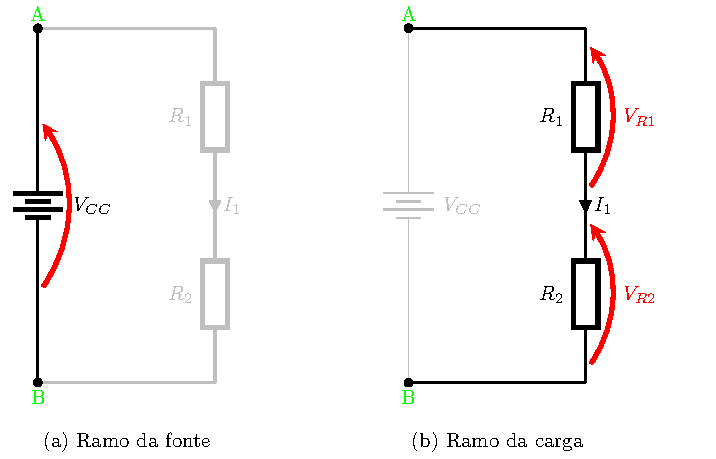
\includegraphics[scale=1.0]{fig-malha}
	\label{fig:malha}
\end{figure}

A segunda lei de Kirchhoff diz que: \textbf{A soma das tensões (ou quedas de tensão) em uma malha é igual a zero}.

Adotando um ponto como referencia de partida, por exemplo o ponto $A$, percorre-se no sentido da corrente, por todo circuito até retornar ao ponto de partida. Ao encontrar uma indicação de tensão no mesmo sentido, adota-o como valor positivo, e no sentido contrário, adota-o como negativo.

Assim, pode-se representar a equação da malha pela definição da seguinte forma:

\begin{eqnarray}
	(-V_{R1}) + (-V_{R2}) + (V_{CC})  & = & 0 \\
	-V_{R1} - V_{R2} + V_{CC} & = & 0 \nonumber\\
	\color{red}{ + \cancel{ V_{R1} } + \cancel{ V_{R2} } } \color{black}{- \cancel{V_{R1}} } - \color{black}{\cancel{ V_{R2}} } + V_{CC} & = & \color{red}{+ V_{R1} + V_{R2}} \nonumber\\
	 V_{CC} & = & V_{R1} + V_{R2}
\end{eqnarray}


Sabemos que em um ramo cada resistor apresenta uma parcela proporcional da resistência total, pois a soma dessas parcelas é a própria resistência total.
\begin{eqnarray}
R_1 + R_2 = R_{T_{ramo}}
\end{eqnarray}

Temos que $R_{T_{ramo}}$ é a resistência total do ramo e é formada por duas partes, $R_1$ e $R_2$, somados. Assim cada resistor é uma parte da resistência total do ramo, um parte do todo.

Sabemos que a parte dividida pelo todo é uma relação de proporcionalidade e que a queda de tensão em cada resistor do ramo é proporcional a sua resistência em relação a resistência total, assim temos que:
\begin{eqnarray}
\frac{R_1}{R_2+R_1} & = & \frac{V_{R1}}{V_{R2}+V_{R1}}\\
\nonumber\\
V_{AB} & = & V_{R1} + V_{R2} \\
\nonumber\\
\frac{R_1}{R_2+R_1} & = & \frac{V_{R1}}{V_{AB}}
\end{eqnarray}
Isolando-se $V_{R1}$  temos:
\begin{eqnarray}
V_{R1} & = & \frac{R_1}{R_2 + R_1} . V_{AB}
\end{eqnarray}
Iguanlmente para $V_{R2}$:
\begin{eqnarray}
V_{R2} & = & \frac{R_2}{R_2 + R_1} . V_{AB}
\end{eqnarray}
